\chapter{Fairness} \label{chap:fairness}
% TODO: Introduction into the chapter, what we want to achieve, that we want try to define what Fairness is and how to measure it.

% TODO: Reword
So far, we have discussed recommender systems and the methods used in the field. We will step back and look at the problem from a broader perspective. Specifically, we want to focus on the importance of fairness and see how and if we can make group recommenders better if we understand it and define it properly.

We will start with a general introduction to the topic of fairness. Define its possible meanings and specify which one is important in our setting. This is required due to the overload of the word itself and the rising importance of the topic in today's world. Further, we will explain why fairness seems to be a crucial parameter in the group recommender setting and will try to reason about how to measure its effects.

\todo[inline]{Notes: If you have enough, why do you care if someone gets more}




\section{General} \label{sec:02_general}
% TODO: Start with a broad overview, why do we need something like fairness, define it, speak about it broadly.
% TODO: Problems with fairness, areas of usage, many possible definitions.

% I want to make an argument, that fairness is important to prevent notions of inequality which inherently leads to negative emotions

% it should lead the reader to think about it more, all the things we are discussing are general knowledge, we are not introducing something crazy

% IDEAS: Mention usage of the word fair/fairness
% https://www.youtube.com/watch?v=dKob6b8QzkU
% monkeys 
% https://www.youtube.com/watch?v=vHE6AYNOCrg
% many meaning of the word fairness, what does it mean for something to be fair

% the notion of fairness is probably important for developing cooperation

The word itself is defined in Cambridge Dictionary \cite{fairness_definition} as "The quality of treating people equally or in a way that is reasonable." Its use has been rising steadily from the 1960s as we can see on \ref{fig:popularity_of_fairness}.

\begin{figure}[htbp]
    \centering
    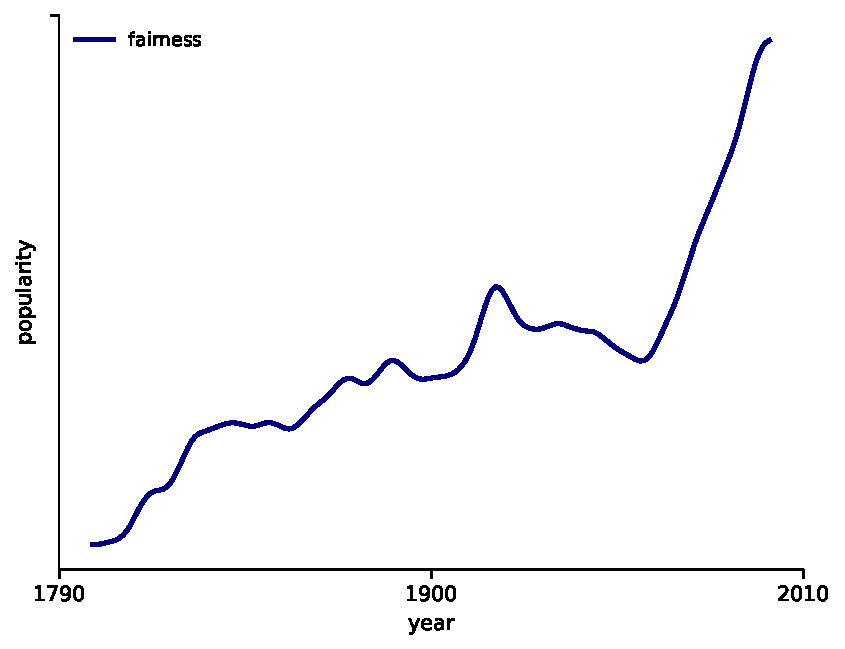
\includegraphics{img/google_ngram_fairness-eng_2012-1800-2000.pdf}
    \caption{The graph shows the phrase 'fairness' occurring in the corpus of English books from 1800 to 2010. Source: Google Ngram Viewer, corpora 2012. \cite{google_ngram_viewer_2012}}
    \label{fig:popularity_of_fairness}
\end{figure}

We, humans, are obsessed with fairness. From a young age, children will get sad when something is not fair, when their sibling gets a more significant piece of a pie, more attention from their parent, or any other unequal situation. It can induce strong emotions such as envy, sadness, or anger, and it emerges very early, as early as 12 months of age or sooner as researched in \cite{children_fairness}.

And this is not limited only to humans; we can observe the same behavior in monkeys. In \cite{brosnan2003monkeys}, the authors observed that if a monkey is getting the worse reward for the same task as its peer,  it refuses the reward and demands the same payout even if they were satisfied with the lesser reward for the same task before.

We observe the same behavior in many other species, but it does not hold for the animal kingdom in general. It seems that it requires a certain level of intelligence for the notion of fairness to emerge. As discussed in \cite{brosnan2014evolution}, based on studies of other non-human species, this evolutionary puzzle can be further dissected into responses to reward distribution among the cooperating group members. Where humans are even willing to seek equalization of outcomes even if it means that they will loose some of their own reward as studied in \cite{willing_to_pay_to_equality}. At the same time, we humans like "free-rides" where we get high rewards for a small amount of work but dislike when someone else gets the same. This directly corresponds with the fairness itself - "It is not fair if someone else gets something we don't.". But that all depends on our personality and the type of relationship involved. Some are, for example, willing to accept that your partner makes more. But that is very subjective and in some cases can lead even to a larger of envy involved.

In some cases we observe a pattern of generosity, where children are willing to make their own sacrifices in order to ensure fairness, so that the other person does not have less than them, as presented in \cite{children_generocity_blake}. The authors studied fairness in multiple cultural settings and found out that this behavior is learned and only present in some cultures.

On the other hand, our society widely accepts the notion of "winner takes all", which can be problematic in itself, for example, in sports and business. In business it directly shapes the distribution of wealth, which is considered one of the main problems of today's world. But discussing the social aspect of fairness is beyond the scope of this thesis.


When it comes to the true nature of fairness on the deepest level, it could even be possible that the notion of fairness emerges together with cooperation and therefore language and communication. It would mean that it is an inherent property of any intelligent agent that is created through an evolutionary process. But more research has to be done, as our understanding of intelligence, consciousness, and related hard to quantify phenomena is lacking.\newline

Let us now get back to fairness in the context of computer systems.


\section{Algorithmic fairness}\label{subsec:02_general.algorithmic_fairness_and_possible_meanings}
% The Emerging Theory of Algorithmic Fairness
We will focus on fairness regarding society or individuals interacting with a computer system. We will not discuss further any meaning of fairness outside of the domain of computer science. This topic steers away from the main goal of defining fairness for the group RS sub-domain, but we think that it is very important topic in general, deserves more spotlight and can be a good middle step to understand specifics of the group RS setting.

\subsection{How can computer be unfair?}
At first, the idea of a machine being unfair may feel strange. How can a computer that has no notion of race or ethnicity discriminate against a group of people? We say, that the algorithm is biased. In the end those who create the algorithms are people. Gathered data that are used to train the algorithm are from the real world. And so they reflect biases that are present in society. Algorithms them selves are not written with ill-fated purpose, it is just a side effect. We can say that the results of any machine learning algorithm are just the product of the underlying data.

It is important to define which sensitive characteristics need to be taken into account. That is a topic for social science to determine, but usually those are: gender, ethnicity, sexual orientation, disability, and so forth.

Research of algorithm fairness tries to analyze machine learning algorithms and data gathering and processing with the goal of understanding how bias in them is created and how it can be fixed.
\newline
As stated in \cite{pessach2020algorithmic_fairness} main sources of unfairness can be:
\begin{itemize}
    \item \textbf{Biases already included in the data set}
    Such as dependence/correlation of data based on sensitive characteristics.
    \item \textbf{Biases caused by missing data}
    Results in dataset that does not represent the target population
    \item \textbf{Biases stemming from algorithmic objectives}\newline
    While training, we usually minimize some error, but that can lead to prioritization of interests of majority.
    \item \textbf{Biases caused by "proxy" attributes}\newline
    When sensitive/private data get removed or replaced, relationship can be created from which algorithm can still deduce the original bias
\end{itemize}


Fairness is studied from the perspective of discrimination in most recent literature into the impacts of algorithms on society. We observe bias to specific groups of population based on their race, sex, nationality, education, beliefs, and many other attributes. And it is essential to study techniques and strategies to mitigate this unfairness.

Further, we can also view fairness from the aspect of algorithmic decision-making, where a decision process can introduce unfairness based on some non-deterministic property or computation. Some sectors such as justice and finance have to strive for equality of outcome due to the high cost of errors or unfair decisions. Either in the form of unjust punishments in the former case or financial loss in the latter one.

The subsequent possible interpretation that applies to our group recommender domain is the notion of fairness in the sense of balance of preference between members of a group. Each member has their preference, and we are trying to balance them in the best possible way so that everyone likes the recommended object or list of objects equally. They may like the recommendation less because their favorite items may not be present.

\subsection{Measures of algorithmic fairness}
We need to have a precise way how to measure bias of the sensitive characteristics. Some of the simple statistical methods presented in \cite{wikipedia-algo-fairness} are:
\begin{itemize}
    \item \textbf{Independence}
    We say that sensitive characteristic S is independent of prediction R if 
    \begin{equation}
        P\left(R = r|S = a\right)=P\left(R=r|S=b\right) \quad \forall r\in R \quad \forall a,b \in S
    \end{equation}
    
    \item \textbf{Separation}
    \item \textbf{Sufficiency}
    
\end{itemize}





%\subsection{X}\label{subsec:02_general.x}


\section{Fairness in Group recommender systems} \label{sec:02_fairness_in_grs}
% TODO: Important to distinguish and define the fairness in the group setting. Other related things such as group dynamics, LONG-TERM fairness, balancing among users. Possible RS related problems.

% Already mentioned in the next chapter, need support for: single item vs list fairness.

We will now focus only on the group RS setting, mentioning some of the main ways how fairness can be understood in this context:

\begin{itemize}
    \item \textbf{Fairness distribution in isolated recommendation}\newline
    We recommend a list of items (possibly even a single item) and have to balance the items that all members will be satisfied by the selection. This single list is an isolated recommendation. We can view fairness in this setting as a direct optimization problem, where items are considered better if they are liked on average (among the group members) more than items liked by some part of the group and disliked by the other. As the group size grows, this is harder and harder to satisfy because a larger group will most probably have a broader preference which will be harder to satisfy.
    
    \item \textbf{Fairness in a list of items that are consumed sequentially}
    This setting differs from the previous because we can be recommending items that are less universally likable but more specific and liked by part of the group. Therefore intertwining the items so that each member will be satisfied "at some point". The balance of group-likable or member-likable items can be tuned according to the specific requirement.
    
    \item \textbf{Long-term fairness}\newline
    Further, we can distinguish another case where recommendations are provided in batches separated by some more significant amount of time (days or longer). This case is somewhat similar to the last one but differs by the fact that unfairness can be more costly to repair. If a person dislikes the item recommended by a group RS, they will less likely be part of the recommendation in the future. So the balance mentioned in the previous setting is an even more important and sensitive parameter to tune. And at the same time, it is more important to gather and process feedback.
    
    \item \textbf{Uneven importance of the group members}
    In some cases, there will be a situation where the expectation of fairness is distributed non-uniformly. For example, when watching a movie with your kids, you probably care about the satisfaction of your kids more than your own. But at the same time, you want to take yourself into account too. In these cases, it is essential to view required fairness as a fluid parameter that can be modified and satisfied by uneven criteria towards group members.
    
    \subsection{Evaluation} \label{sec:02_evaluation}
% TODO: It is nice to see what we want, but in order to build algorithms and improve, we first need to know how to measure it. List possible ways of how to measure the fairness, mainly in regards to group recommenders. Then discuss about the evaluation on data. The exact process of processing the the training and testing. Define everything very precisely and rigorously.
    
\end{itemize}

\section{Other properties} \label{sec:02_other_properties}
Let us now discuss some similar properties that are closely tied together with fairness in the general setting and algorithmic setting as it it crucial to have wide overview of the problem in order to design algorithms that optimize fairness it self. We can have a fair algorithm, but to what use it will be, if it recommends bad items that are disliked. Fairness inherently has to be part of a multi-criterion optimization.

\subsection{Bias}
As already mentioned before, bias is an important property that we are trying to suppress. Examples of bias are all around us. Each person has at least some prejudice and ideas about topics that they are not familiar with or that society is giving them. It is therefore important that we actively try to broaden our minds and suppress these biases. Just then, we can truly become equal as individuals.

From the algorithmic view, bias is mostly introduced with the underlying data, that we process. Sometimes these biases are used to even generate profit. For example marketing, where sex is a very good indicator of preference. A good question arises - where lies the line between fair usage and abuse? We don't know yet, but it seems that privacy and fairness will be gaining importance and therefore the question of how to get rid of bias will become more significant.


\subsection{Similarity}


\subsection{Privacy}
\subsection{Integrity}
\subsection{Legitimacy}

\subsection{Accuracy}
\subsection{Precision}
\subsection{Coverage}
\subsection{Diversity}
\subsection{Novelty}



% TODO: Fairness is not the only property we can try to manage, what about privacy, accuracy, precision, coverage, diversity, novelty and so on. Mention them first in an overview, then separately in subsections in more detail. Try to define them mathematically.
